\documentclass[12pt]{article}
\usepackage[italian]{babel}
\usepackage{geometry}
\usepackage{amsmath}
\usepackage{amssymb}
\usepackage{graphicx}
\usepackage{ulem}

\geometry{margin=2cm}
\let\olditemize\itemize
\renewcommand\itemize{\olditemize\setlength\itemsep{0em}}

\title{Esercizi - Modello Relazionale}
\author{Lorenzo Vaccarecci}
\date{7 Marzo 2024}

\graphicspath{{../Immagini/}}

\begin{document}
\maketitle
\section{Esercizio}
\textbf{Domanda: }\textit{Quante chiavi esterne può contenere una relazione?}
\\Opzioni:
\begin{itemize}
    \item  $\boxtimes$ una
    \item  $\boxtimes$ nessuna
    \item  $\boxtimes$ più di una
\end{itemize}
\section{Esercizio}
\textbf{Domanda: }\textit{Data la seguente relazione $R$ con chiave $A_{i}$ e una relazione $R'(\uline{B_{1}},B_{2}^R)$ quali delle sueguenti istanze $R'$ violano l'integrità referenziale?}
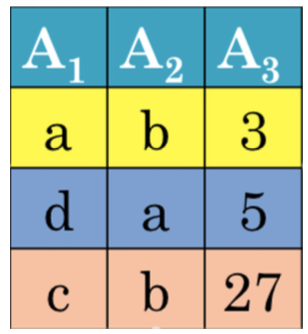
\includegraphics[width=0.2\textwidth]{esercizio2.png}
\\Opzioni:
\begin{itemize}
    \item $\boxdot$ $\emptyset$
    \item $\boxdot$ $\{(1,a)\}$
    \item $\boxtimes$ $\{(2,b)\}$
    \item $\boxdot$ $\{(1,a),(3,c),(4,d)\}$
    \item $\boxtimes$ $\{(1,a),(2,b),(3,c),(4,d)\}$
\end{itemize}
\section{Esercizio}
\textbf{Domanda: }\textit{Data la relazione Cliente(\uline{codCli},nome,cognome,telefono,dataN,residenza) quali delle seguenti sono definizioni corrette di relazione che riferisce Cliente?}
\\Opzioni:
\begin{itemize}
    \item $\boxtimes$ Nol(collocVideo, dataNol, cliente$^\text{Cliente}$, dataRest$_{o}$)
    \item $\boxtimes$ Nol(collocVideo, dataNol, codCli$^\text{Cliente}$, dataRest$_{o}$)
    \item $\boxtimes$ Nol(collocVideo, dataNol, minnie$^\text{Cliente}$, dataRest$_{o}$)
    \item $\boxdot$ Nol(collocVideo, dataNol, nomeCli$^\text{Cliente}$, cognomeCli$^\text{Cliente}$, dataRest$_{o}$)
\end{itemize}
\section{Esercizio}
\textbf{Domanda: }\textit{Data una relazione $R$ con una sola chiave $A,B$}
\begin{itemize}
    \item $\boxtimes$ ogni chiave esterna su $R$ dovrà contenere due attributi
    \item $\boxdot$ ogni chiave esterna su $R$ dovrà contener gli attributi $A$ e $B$
    \item $\boxdot$ per fare riferimento a $R$ si potrà utilizzare $A$ oppure $B$
\end{itemize}
\section{Esercizio}
\textbf{Domanda: }\textit{Sia $FK$ un insieme di attributi definiti come chiave esterna in una relazione $R$}
\begin{itemize}
    \item $\boxdot$ $FK$ è certamente una chiave di $R$ 
    \item $\boxtimes$ $FK$ può essere una chiave di $R$ 
    \item $\boxdot$ $FK$ è certamente un sottoinsieme proprio di una chiave di $R$ 
    \item $\boxtimes$ $FK$ può essere un sottoinsieme proprio di una chiave di $R$ 
    \item $\boxdot$ $FK$ è certamente disgiunto da tutte le chiavi di $R$ 
    \item $\boxtimes$ $FK$ può essere disgiunto da tutte le chiavi di $R$
\end{itemize}
\section{Esercizio}
\textbf{Consegna: }\textit{Si consideri il seguente schema relazionale, relativo ad una casa editrice di riviste di settore}
\\ RIVISTA(\uline{CodR}, Nome, Tipo, Direttore$^{AUTORE}$)
\\ ARTICOLO(\uline{CodA}, Titolo, Argomento, Lunghezza, CodU$^{AUTORE}$,CodR$^{RIVISTA}$, DataPubblicazione)
\\ AUTORE(\uline{CodU}, Nome, Cognome, Tel, ComuneResidenza)
\\ LAVORA(\uline{CodR$^{RIVISTA}$}, \uline{CodU$^{AUTORE}$}, DataI)
\begin{itemize}
    \item Uno stesso articolo può essere pubblicato in riviste diverse? NO
    \item Uno stesso articolo può essere pubblicato più volte nella stessa rivista? NO
    \item Articoli con lo stesso titolo possono comparire più volte nella stessa rivista? SI
    \item Articoli con lo stesso titolo possono comparire su riviste diverse? SI
    \item Un articolo può avere più di un autore? NO
    \item Un autore può firmare più articoli nella stessa rivista? SI
    \item Un autore può firmare più articoli in riviste diverse? SI
    \item Una rivista può avere più direttori? NO
    \item Un direttore può dirigere più riviste? SI
\end{itemize}
\textbf{Consegna: }\textit{Mostrare una possibile istanza della relazione LAVORA che violi il vincolo di chiave primaria}
\\ LAVORA($\emptyset$, xx, xx/xx/xxxx) oppure\\ LAVORO(12, 35, xx/xx/xxxx) e LAVORO(12, 35, xx/xx/xxxx)
\\\textbf{Consegna: }\textit{Mostrare una possibile istanza della relazione RIVISTA ed un'istanza della relazione AUTORE che violino i vincoli di chiave esterna}
\\ AUTORE($\emptyset$)
\section{Esercizio}
\textbf{Consegna: }\textit{Si consideri il seguente schema relazionale:}\\
Pizza(\uline{codP}, nome, prezzo)\\
Ingrediente(\uline{codP$^{Pizza}$, ingrediente})\\
Cliente(\uline{telC}, cognomeC, nomeC, via, nCiv, nInt)\\
Ordine(\uline{telC$^{Cliente}$, data, codP$^{Pizza}$}, qta, importo)\\
\textbf{Consegna: }\textit{Se sappiamo che la relazione Pizza contiene 25 tuple e la relazione Ordine ne contiene 200}
\begin{itemize}
    \item Quante tuple può contenere la relazione Ingrediente
    \begin{itemize}
        \item \textbf{Risposta: } [0, $n$] con $n$ numero grande ma finito (la tabella potrebbe non essere piena)
    \end{itemize}
    \item Quante tuple può contenere la relazione Cliente
    \begin{itemize}
        \item \textbf{Risposta: } [1, $n$] con $n$ numero grande ma finito (un cliente potrebbe non aver ordinato)
    \end{itemize}
\end{itemize}
\end{document}